%===================================================================================
% Chapter: Metodologia
%===================================================================================
\chapter{Metodología}\label{chapter:metodologia}
%\addcontentsline{toc}{chapter}{Marco Teórico}
%===================================================================================

En este capítulo se describe la metodología y la estructura empleada en la implementación de un simulador computacional del sistema inmune de un lactante para modelar la respuesta a vacunas conjugadas neumocócicas.

El simulador se estructura en dos capas principales:
\begin{enumerate}
    \item Modelado de agentes biológicos:
        \begin{enumerate}
            \item Antígenos
            \item Células B
        \end{enumerate}
    \item Entornos de Interacción:
        \begin{enumerate}
            \item Centros germinales
            \item Sistema inmune
        \end{enumerate}
\end{enumerate}
\section{Modelado de agentes biológicos}
\begin{enumerate}
    
    \item \texttt{Antígeno}: Representado por un vector de epítopos, cantidad de polisacárido, proteína portadora y factor de inmunogenicidad.
    \item \texttt{Célula B}: 
    Representada por un identificador, un vector de receptores, un serotipo asociado que representa el antígeno que ha reconocido y una afinidad por este.
\end{enumerate}

    


\section{Centros Germinales}

Los centros germinales constituyen conglomerados de células B que reconocen el mismo antígeno en los cuales estas se dividen rápidamente.
\subsection*{Procesos Inmunológicos clave}
En los centros germinales ocurren procesos en función de la especialización y diferenciación de las células B.
\begin{enumerate}
    \item \textbf{Cálculo de afinidad:}

    La afinidad entre una célula B y un antígeno es una medida fundamental que cuantifica la fuerza de interacción entre el receptor de la célula B (BCR por sus siglas en inglés) y el epítopo del antígeno. Este cálculo se basa en la similitud estructural entre sus vectores característicos, modelados en un espacio n-dimensional donde cada dimensión representa una propiedad fisicoquímica relevante (como carga eléctrica, hidrofobicidad o tamaño molecular).

    Definimos la afinidad $A$ mediante la transformación exponencial de la distancia euclidiana entre los vectores:

    \begin{equation}
    A = e^{-d(\vec{r}_{B}, \vec{e}_{A})} = \exp\left({-||\vec{r}_{B} - \vec{e}_{A}||}\right)
    \end{equation}

    donde:
    \begin{itemize}
        \item $\vec{r}_B \in \mathbb{R}^n$ es el vector característico del receptor de la célula B, que codifica las propiedades moleculares de su sitio de unión.
        
        \item $\vec{e}_A \in \mathbb{R}^n$ es el vector característico del epítopo antigénico, representando sus características estructurales clave para el reconocimiento inmunológico.
        
        \item $d(\vec{r}_{B}, \vec{e}_{A}) = ||\vec{r}_{B} - \vec{e}_{A}||$ es la distancia euclidiana en $\mathbb{R}^n$, calculada como:
        \begin{equation}
        d = \sqrt{\sum_{i=1}^{n} (r_{B,i} - e_{A,i})^2}
        \end{equation}
        
        \item $A \in (0,1]$ es la medida de afinidad resultante.
    %     , con propiedades biológicamente significativas:
    %     \begin{itemize}
    %         \item \textbf{Valor 1}: Máxima afinidad (vectores idénticos, distancia = 0)
    %         \item \textbf{Valores cercanos a 0}: Baja afinidad (vectores disímiles)
    %         \item \textbf{Función monótonamente decreciente}: Mayor distancia $\Rightarrow$ menor afinidad
    %     \end{itemize}
    \end{itemize}

    % \textbf{Interpretación biológica:} Esta formulación captura dos principios esenciales de las interacciones inmunológicas:
    % \begin{enumerate}
    %     \item La \textbf{complementariedad estructural} entre el BCR y el epítopo determina la fuerza de unión
    %     \item La relación no es lineal: pequeñas diferencias estructurales en regiones críticas pueden causar grandes disminuciones en la afinidad (propiedad emergente de la función exponencial)
    % \end{enumerate}

    % \textbf{Ventajas computacionales:}
    % \begin{itemize}
    %     \item Normalización intrínseca ($0 < A \leq 1$)
    %     \item Diferenciabilidad para algoritmos de optimización
    %     \item Penalización exponencial de disparidades estructurales
    %     \item Eficiencia de cálculo con operaciones vectorizadas
    % \end{itemize}
    \item \textbf{Selección de células B mediante distribución de Boltzmann:}

La selección de las células B que sobreviven en cada generación se realiza mediante un algoritmo estocástico basado en la distribución de Boltzmann, que asigna probabilidades de supervivencia proporcionales a la afinidad de cada célula mientras mantiene diversidad poblacional. Este proceso consta de tres etapas:

\begin{enumerate}
    \item \textbf{Cálculo de probabilidades:} Para cada célula B con afinidad $A_i$, se calcula una probabilidad de supervivencia:
    \[
    P_i = \frac{e^{A_i / T}}{\sum_{j=1}^{N} e^{A_j / T}}
    \]
    donde:
    \begin{itemize}
        \item $T$ es el parámetro de temperatura que regula la presión selectiva
        \item $N$ es el tamaño total de la población
        \item $A_i \in [0,1]$ es la afinidad de la célula $i$
    \end{itemize}
    
    \item \textbf{Normalización numérica:} Para evitar inestabilidades computacionales, se aplica una transformación estable:
    \[
    A_i^{\text{norm}} = A_i - \max_{j}(A_j)
    \]
    garantizando valores negativos o cero sin alterar las proporciones relativas.
    
    \item \textbf{Muestreo estocástico:} Se seleccionan $K$ células sin reemplazo según:
    \[
    \text{Seleccionados} \sim \text{Multinomial}(K; P_1, P_2, \dots, P_N)
    \]
    donde $K = \min(\text{max\_survivors}, N)$ modela restricciones de recursos.
\end{enumerate}

\noindent \textbf{Interpretación de parámetros:}
\begin{itemize}
    \item \textbf{Temperatura (T):} Regula el balance diversidad-optimización:
    \begin{itemize}
        \item $T \to 0^+$: Selección elitista (solo células con máxima afinidad)
        \item $T \to \infty$: Selección aleatoria uniforme (máxima diversidad)
        \item $T \approx 0.5$: Balance biológico típico en simulaciones
    \end{itemize}
    
    \item \textbf{max\_survivors:} Modela restricciones biológicas:
    \begin{itemize}
        \item Espacio en nichos linfoides
        \item Disponibilidad de factores de crecimiento
        \item Capacidad de presentación antigénica
    \end{itemize}
\end{itemize}

% \noindent \textbf{Base biológica:} Este modelo captura mecanismos esenciales de selección clonal:
% \begin{itemize}
%     \item \textbf{Supervivencia diferencial:} Células con mayor afinidad tienen mayor probabilidad de persistir
%     \item \textbf{Preservación de diversidad:} Permite la supervivencia de células con afinidad subóptima pero potencial evolutivo
%     \item \textbf{Competición por recursos:} El muestreo sin reemplazo simula limitaciones del microambiente
% \end{itemize}

% \noindent \textbf{Ventajas computacionales:}
% \begin{itemize}
%     \item Diferenciabilidad para métodos basados en gradiente
%     \item Complejidad $O(N)$ eficiente para grandes poblaciones
%     \item Control preciso de presión selectiva mediante $T$
%     \item Implementación estable con normalización exponencial
% \end{itemize}
    \item \textbf{Diferenciación:}
    
    Según su afinidad, las células B pueden diferenciarse en:
        \begin{enumerate}
            \item Células de memoria 
            \item Células plasmáticas 
        \end{enumerate}
    \item \textbf{Hipermutación somática de células B:}

El proceso de mutación simula la hipermutación somática que ocurre en los centros germinales durante la respuesta inmune adaptativa. Cada componente del vector receptor $\vec{r}_B$ de una célula B tiene una probabilidad $p_m$ de sufrir una modificación estocástica, modelada como:

\begin{equation}
r_i' = \text{clip}\left(r_i + \delta_i, 0, 1\right) \quad \text{donde} \quad \delta_i \sim 
\begin{cases} 
\mathcal{N}(0, \sigma^2) & \text{con probabilidad } p_m \\
0 & \text{en caso contrario}
\end{cases}
\end{equation}

\noindent \textbf{Parámetros clave:}
\begin{itemize}
    \item \textit{Tasa de mutación ($p_m$)}: Probabilidad de que un componente individual mute (valores típicos: 0.05-0.15). Biológicamente, refleja la actividad de la enzima AID (citidina desaminasa) en linfocitos B.
    
    \item \textit{Intensidad de mutación ($\sigma$)}: Desviación estándar de la distribución gaussiana que determina la magnitud de las alteraciones (valores típicos: 0.01-0.1). Modela el impacto estructural de las mutaciones puntuales.
\end{itemize}

\noindent \textbf{Procesamiento post-mutación:}
\begin{itemize}
    \item \textit{Normalización de valores:} Los componentes se limitan al intervalo $[0,1]$ mediante:
    \[
    \text{clip}(x, a, b) = \max(a, \min(x, b))
    \]
    garantizando vectores biológicamente plausibles.
    
    \item \textit{Reseteo de afinidad:} La afinidad de la célula mutada se inicializa a cero, requiriendo recálculo contra antígenos.
    
    \item \textit{Preservación de linaje:} Se mantienen el identificador único y serotipo para rastreo evolutivo.
\end{itemize}

\noindent \textbf{Base biológica:} Este modelo captura tres propiedades esenciales de la hipermutación somática:
\begin{enumerate}
    \item \textit{Localidad:} Mutaciones puntuales que modifican ligeramente el paratopo
    
    \item \textit{Independencia:} Cada residuo muta de forma autónoma
    
    \item \textit{No direccionalidad:} Los cambios son estocásticos, no guiados por el antígeno
\end{enumerate}

\noindent \textbf{Implementación computacional:}
\begin{itemize}
    \item \textit{Vectorización:} Uso eficiente de operaciones NumPy para grandes poblaciones
    
    \item \textit{Modelo de mutación aditiva:} Alteraciones gaussianas independientes por componente
    
    \item \textit{Generación de nuevas variantes:} Creación de instancias modificadas sin alterar células originales
\end{itemize}

\noindent \textbf{Contexto evolutivo:} Combinado con selección de Boltzmann, este mecanismo permite:
\begin{itemize}
    \item Exploración local del espacio de receptores alrededor de soluciones prometedoras
    
    \item Escape de óptimos locales mediante mutaciones beneficiosas
    
    \item Mantenimiento de diversidad clonal durante la respuesta inmune
\end{itemize}

% \noindent \textbf{Ejemplo numérico:} Para un receptor $[0.8, 0.5]$ con $p_m=0.1$, $\sigma=0.05$:
% \begin{itemize}
%     \item Componente 1: No muta (prob $>0.1$) $\rightarrow 0.8$
%     \item Componente 2: Mutación con $\delta = +0.03$ $\rightarrow 0.53$
%     \item Receptor mutado: $[0.8, 0.53]$
% \end{itemize}
\end{enumerate}

Las células B ingresan al centro germinal tras calcular su afinidad inicial con el antígeno. Dentro del mismo, el proceso de selección identifica las células candidatas para abandonarlo, las cuales se diferencian en células plasmáticas o de memoria antes de reintegrarse al sistema inmunológico. Las células no seleccionadas enfrentan dos destinos posibles: muerte por apoptosis (pérdida energética), o supervivencia con división y mutación. Para este último grupo, se aplica hipermutación somática a sus receptores y se recalcula su afinidad antigénica, reiniciando el ciclo, como se muestra en la figura \ref{fig:cg}. Este proceso iterativo continúa hasta la desaparición de todas las células del centro germinal. 

\begin{figure}[H] % h = here (aquí)
    \centering
    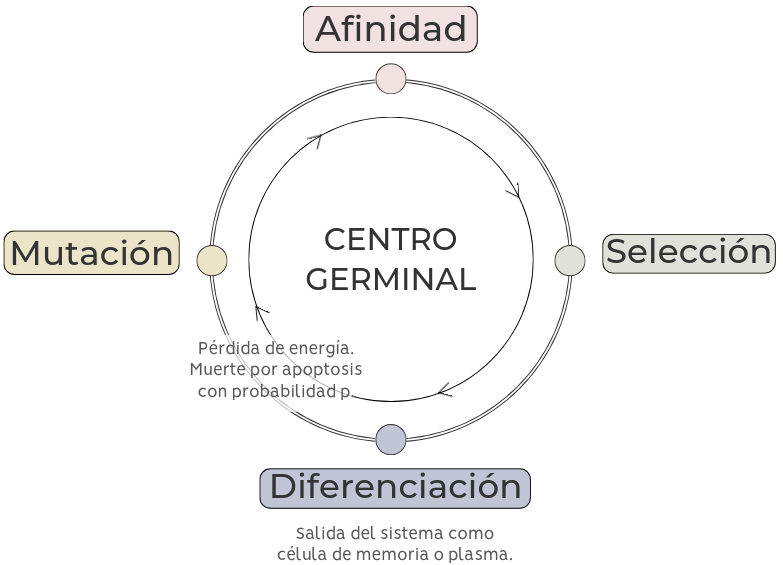
\includegraphics[width=1\textwidth]{Graphics/gc.png}
    \caption{Ciclo que ocurre dentro del Centro Germinal}
    \label{fig:cg}
\end{figure}

\section{Sistema Inmune}

El sistema inmune consta de un grupo de células B \textit{naive} que se dividen y mutan o mueren. Ante la presencia de antígeno estas células pueden pasar a formar parte de centros germinales como se muestra en la figura \ref{fig:is}. 

Al finalizar cada ciclo, los centros germinales liberan al sistema inmunológico células B diferenciadas en células plasmáticas y células de memoria. La concentración de anticuerpos generada por estas sirve como indicador cuantitativo de la respuesta inmunológica del individuo.

\begin{figure}[H] % h = here (aquí)
    \centering
    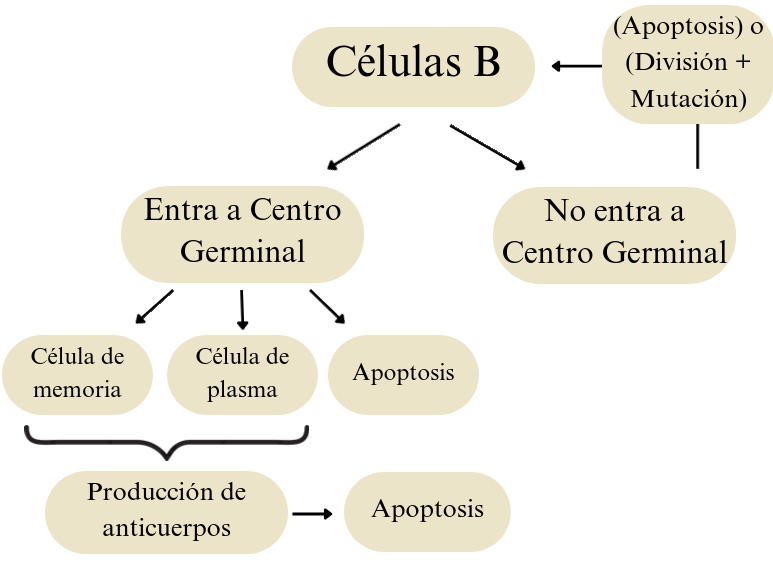
\includegraphics[width=1\textwidth]{Graphics/is.png}
    \caption{Células B dentro del sistema inmune}
    \label{fig:is}
\end{figure}




% aaaaaaaaaaaaaaaaaaaaaaaaaaaaaaaaaaaaaaaaaaaaaaaaaaaaaaaaaaaaaaaaaaaaaaaaaaaaaaaaaaa
% aaaaaaaaaaaaaaaaaaaaaaaaaaaaaaaaaaaaaaaaaaaaaaaaaaaaaaaaaaaaaaaaaaaaaaaaaaaaaaaaaaa
% aaaaaaaaaaaaaaaaaaaaaaaaaaaaaaaaaaaaaaaaaaaaaaaaaaaaaaaaaaaaaaaaaaaaaaaaaaaaaaaaaaa
% aaaaaaaaaaaaaaaaaaaaaaaaaaaaaaaaaaaaaaaaaaaaaaaaaaaaaaaaaaaaaaaaaaaaaaaaaaaaaaaaaaa
% aaaaaaaaaaaaaaaaaaaaaaaaaaaaaaaaaaaaaaaaaaaaaaaaaaaaaaaaaaaaaaaaaaaaaaaaaaaaaaaaaaa


